



\chapter{Introduction}\label{ch:introduction}
\section{Ultrasound contrast using two acoustic waves}\label{sec:int:Introduction}

 

 

% \missingfigure{Add my picture here.}
Ultrasound uses the {\em pulse-echo transit time} of a sound pulse -
the time interval between the pulse being emitted and returning again -
to measure the depth at which an acoustic reflection occurred.
The strength of the returned signal is plotted
%\footnote{Often it is actually the 'brightness' of the signal that is plotted.
%This is the envelope of the returned signal,
%often achieved with a Hilbert transform.}\todo{fix this footnote}
against this depth to form an image of the echo characteristics of the material.

%Micron-sized bubbles have been used since ...\todo{find the year}\cite{} 
%to improve the signal strength from echo poor regions


The echos returned from micron sized bubbles ({\em microbubbles}) are stronger than from most biological structures.
%and this property means that when they are introduced into a patient they enhance contrast.
This is because the incident sound wave induces radial pulsations in the gas bubbles
which then become acoustic sources themselves.
The pulsations are resonant when insonated at diagnostic frequencies (\unit{1-10}\mega\hertz).
%and their normalised scattering cross sections can reach order $10^5$ \todo{check order of scattering xs}\cite{}.
When microbubbles are injected into a patients blood
they increase the strength of the echo
from a tissue-type that is otherwise echo poor.
Injected microbubbles thereby act as a contrast agent for diagnostic ultrasound,
and have been used in this way since 1994\cite{NYtimesAlbunex}.
%Microbubbles  form secondary acoustic sources. %that can be identified and be used to enhance contrast.

%\todo[inline]{And another one.}
%Often the sound returns due to changes in acoustic impedance
%that result from a local variation in sound speed.
%Alternatively the sound can induce resonances in structures within the body which then act as acoustic sources.
%This does not occur naturally at diagnostic frequencies (\unit{1-10}\mega\hertz).
%However, 
%the radial pulsations of micron-sized gas bubbles  are resonant when insonated with ultrasound
%and 
%{\em microbubbles} may therefore be injected into the body and identified. 
%They have been used as ultrasound contrast agents since 19.. (cite).
%They improve the signal generated from echo-poor tissue types,
%and may be functionalised to target specific molecular
%markers (cite).

The application of microbubble imaging is limited to the blood, however, by the bubble's size.
The largest diameters that may be  moved across endothelial cells (via {\em vesiculo-vacuolar transport}) are approximately \unit{150}\nano\metre\cite{Hobbs1998},
ten times smaller than the average microbubble.
Other trans-cellular transport mechanisms are still more limiting,
with potocytosis being able to transfer diameters of approximately \unit{50}\nano\metre\cite{Anderson1993,Khalil2006}.
Conventional microbubbles are also too large to pass through `leaky' tumour vasculature, where gaps of between \unit{300-600}\nano\metre\ can be found between endothelial 
cells\cite{Fukumori2006, Hashizume2000,  Hobbs1998}.
%although if should also be noted the rarity and distribution of such gaps is not entirely clear\cite{Hashizume2000}.


The development of a bubble contrast agent much smaller than $\unit{0.5}\micro\metre$ has not been forthcoming.
One difficulty is stability.
As the bubble is shrunk the  Laplace pressure within the bubble, and with it the chemical potential, 
grows rapidly.
The bubble then equilibrates  by dissolving.
This effect can be mitigated by the use of an encapsulating shell\cite{Ferrara2007}.
However, the difficulty then is that the resulting bubbles tend to be very stiff, 
and so inducing them to pulsate becomes hard\cite{Bloch2005,Zhanwen2010,Borkent2007}.
Generating stable \unit{100}\nano\metre\  bubbles that can be used for ultrasound imaging has proven challenging,
although there are recent signs of success\cite{Zhanwen2010}.

Since microbubbles are currently limited to the blood 
they do not from a good general purpose contrast agent.
It is beyond the capabilities of diagnostic ultrasound
to image a particular type of tissue,
or to image a particular chemical environment within a tissue.
To image such biological function other modalities must be used,
such as  
functional MRI\cite{Lanza2004a},
quantum dots\cite{Ballou2004} or
opto-acoustic imaging with a gold nanoparticle contrast agent\cite{Copland2004}.
However, each of these modalities have their own short-comings,
be they image resolution, time of image acquisition, 
invasiveness of the imaging procedure, 
health risks associated with the contrast agent,
or cost.
Ultrasound offers real-time imaging with millimetre precision
in a safe, cost-effective and relatively uninvasive procedure.
Its lack of functional imaging is a real loss.

There is a second problem that is caused by the lack of submicron bubbles.
To attain good contrast the frequency of the ultrasound pulse should match
the resonance frequency of the bubbles.
This increases as the bubbles get smaller\cite{Zheng2006}.
The lack of submicron bubbles means that there is no adequate contrast agent at the micron-scale resolutions attainable by high-frequency ultrasound imaging (20-\unit{100}\mega\hertz).

%one that is able to image tissue beyond the blood and vasculature.
%that is capable of leaving the blood.
The aim of this thesis is to extend the capabilities of diagnostic ultrasound
by using a second acoustic wave.
This wave has two roles:
%will be used to manipulate a bubble in preparation
%of the primary imaging pulse.
%The manipulation will come in two forms:
\nlist{
  \item generate a bubble in preparation of the imaging wave,
  \item temporarily grow or shrink a bubble so that its resonance frequency better matched to the 
frequency of the imaging pulse.
}
The term {\em driving wave} will be used for the pulse that affects this control over the bubble.

The limitations of ultrasound contrast imaging are greatly reduced
by being able to control the bubble in these ways.
Firstly, a generated bubble can be imaged immediately and so does not have to be stable.  
The lifetime of  a 10-\unit{100}\nano\metre\ bubble without a shell is between 1-\unit{100}\micro\second\cite{Ljunggren1997}, 
a temporal resolution that is well within the capabilities of ultrasound.
Secondly, by controlling the size of the bubble, 
the driving wave also controls the bubble's resonance frequency.
The high frequency response of conventional microbubble imaging 
can be extended by ensuring that the bubble is imaged 
when it has been transitively shrunk by the driving wave.
%timing the imaging wave to be incident upon the bubble
%at such time when the bubble has been shrunk by the driving wave.



Two broad approaches to acoustically generate a microbubble will be considered:
\nlist
{
\item use the reduction in pressure of the driving rarefactions to free a pocket of gas from a mote within the medium.
The mote is the contrast agent in this approach.
\item vapourise an oil based contrast agent.  

There are two mechanisms by which the driving wave can induce the vapourisation.
The reduction in pressure in the driving rarefactions is one possibility.
The heating induced by the driving wave is the other.
Recent experiments using long driving pulse trains with perfluoropenatane droplets,
a perfluorocarbon with a boiling point of approximately 28\degree\cite{Burns2010}, 
seem to favour the second explanation.
It was found that the vapourisation is more easily induced at higher frequencies\cite{Burns2010},
which is the opposite finding to what would be expected if the change was induced by a reduction in pressure. 
Other groups favour the first explanation\cite{Kripfgans2000,Rapoport2007}.

%In this thesis we also investigate perfluoropentane but we shall concentrate on the first mechanism,
%in particular with respect to experimental work.
%Instead of using high-frequency bursts consisting of many cycles,
%we use a relatively short, low frequency pulse with 10-cycles at \unit{0.5}\mega\pascal.
%Perfluoropentane is used because, like the other members of the perfluoroalkane series,
%it is chemically inert, has an unusually low boiling point and an unusually high solubility for gasses such as carbon dioxide.
%The first of these properties causes the perfluoroalkanes to have low toxicity
%and the latter two are encouraging from the perspective of nucleation.
}




%which may then be imaged in the conventional way.
%Conventional wisdom states that 
%lower  frequencies are better at  generating the bubbles (they have a higher mechanical index) whereas higher frequencies give better resolution for imaging.
%(However, Peter Burns has found the opposite for perfluoropentane droplets \cite{Burns2010}, however).
%Therefore two waves will in general be required:
%\nlist{
%  \item a low frequency {\em cavitating wave}  or  {\em driving wave} that generates the bubble.  
%    The driving wave will cause the bubble to  pulsate after it has been created.
%  \item a higher frequency  {\em imaging wave} that is timed to image the bubble while it exists.
%} 


%A liquid droplet solves many of the stability problems of small vapour bubbles.
%It has more molecules than a vapour bubble of the same size, and so does not dissolve so quickly.
%This means that it can be made smaller than a bubble, although actually making droplets of 100-\unit{200}\nano\metre\ remains  challenging.
%The generated bubble will not be stabilised with a shell and so will have a short lifetime.
%This is no longer a problem, however, for the bubble can now be imaged immediately.
%For example, the lifetime of  an unstabilised 10-\unit{100}\nano\metre\ bubble is between 1-\unit{100}\micro\second\cite{Ljunggren1997}.
%Such temporal resolutions are well within the capabilities of ultrasound.
% although may force
%the two waves   to be incident on the droplet/bubble simultaneously.
%
%although the two waves, the cavitating and the imaging waves, 
%may be forced to be coincident on the bubble at the same time.

%although the two waves
%For example, the lifetime of an unstabilised 10-\unit{100}\nano\metre\ bubbles is between 1-\unit{100}\micro\second\cite{Ljunggren1997}.
%This requires that the two waves image the droplet/vapour bubble at the same time or at least in quick succession, but is not a problem in principle.
%The generated vapour bubbles will in general be larger than this.


%However, the generation of the bubble does bring issues of its own.
%The first is the nucleation of the bubble with diagnostic pressures.
%The small volumes of the droplets make  heterogeneous nucleation events unlikely.
%%that enables water to cavitate so easily.
%Homogeneous nucleation, by contrast, usually requires much greater effort.
%The choice of the oil droplet needs careful consideration.
%The desired properties cannot simply be scaled from the properties of water, 
%since we can expect the nucleation mechanisms to be  different.

%The second problem is that the bubbles form explosively  and therefore have, in general, short lifetimes.
%The bubbles are generated in a much more hostile environment than is generally used for contrast imaging,
%where explosive growth in the bubble is  avoided.
%The generated bubble may  collapse and shatter under the influence of the driving wave, 
%or may simply  re-condense rapidly.
%The imaging wave therefore needs to be coincident with the bubble at the time that the bubble is created,
%a time when the driving wave is still present.
%Since the bubble does not respond to the impinging acoustic waves in a linear fashion, 
%the response to the imaging wave will not be independent of the driving wave.

%This final property can be viewed as an opportunity.
%Since the response to the imaging wave also depends on the driving wave,
%the driving wave can be used   to manipulate the bubble to maximise the high frequency scatter.
%For example, it may be used to shrink a large bubble or expand a small bubble towards the high-frequency resonance.

%This thesis investigates these issues in detail.


% This thesis takes a broad approach to the use of an oil droplet as an acoustically generated microbubble.
% We consider the three 

% % The applicability of a liquid droplet should be greater than that of a vapoThe liquid droplet helps the contrast agents
% % Also, since the liquid droplet that we start from has more molecules than a vapour droplet of the same size, 
% % it does not dissolve on the same short timescales.
% % While it is challenging to 

% The use of ultrasound to generate a bubble within the patient has seen a great growth in interest.




% At high pressures microbubbles behave highly non-linearly.
% Imaging the bubble
% The short lifetime encourages 




% This thesis address the following 
% The first is the actual generation of the microbubbles at diagnostic pressures.
% To be able to locate a contrast
% This is difficult because the
% The first is the potential  damage to cells caused initiating widespread cavitation within a small volume. (See Leighton\cite{LeightonBook} for a discussion).
% The second is 
% the rapid expansion of a bubble being formed can damage cells\cite{LeightonBook}



%Generating the bubbles acoustically circumvents both the need for long-lived bubbles,
%for they can be imaged as they are generated,
%and the difficulty in vascularisation.


%To vapourise a portion of  fluid with sound we may attempt to either increase its temperature
%or decrease its pressure.
%\nlist{
%\item increase its temperature,
%\item decrease its pressure.
%}
%The temperature increase will be concentrated at locations where there is an increase in acoustic impedance.
%This roughly correlates with a material region with a slower speed of sound than the bulk.%
%A sound wave, by its very nature, is associated with a fluctuating pressure.
%As the sound wave passes there will be transient decreases in pressure.
%
%
%To ease the vaporisation an oil emulsion that is physically volatile but chemically inert may be used as the medium.
%Perfluoropentane, which is non-toxic and has a boiling point
%of $28^{\text o}$, is chosen to be the oil from which the emulsions
%are to be made.%
%
%Increasing the temperature of a fluid is certainly  possible with ultrasound,
%and is a principle mechanism of High Intensity Focused Ultrasound (\hifu) therapy 
%(cite).
%However, heating requires long pulse trains  (hundreds of pulses),
%which  diagnostic scanners are not in general capable of generating,
%and are associated with significant   bioeffects (cite). % of ultrasound increase with the pulse-length.
%In this thesis therefore, 
%we restrict attention to vapourising pulses that are short (\unit{10}\ cycles or fewer).

\section{Thesis Outline}

The thesis is divided into \ref{part:discussion} parts.
%\Partref{maths} is devoted to the mathematical tools that are used in this thesis.
%\Chapref{gc} introduces David Hestenes' Geometric Calculus that 
%so simplifies the theory of acoustic measurement of \chapref{measurement}.
%\Chapref{inference} introduces the topics of probability, 
%inference and statistical physics that are used 
%in the analysis of acoustic nucleation in \partref{theory}
%and in  analysing the experimental results of \partref{experimental}.
%Nothing but the presentation is novel in these chapters,
%and so they may be skipped if their contents is familiar to the reader.
%%
%
%If the bubble is generated by vaporising an oil droplet then many of the stability problems of small vapour bubbles are also resolved.  
%An oil droplet has more molecules than a vapour bubble of the same size and so does not dissolve so quickly.
%It can therefore be made smaller. % although actually making droplets of 100-\unit{200}\nano\metre\ remains  challenging\cite{}.
%
%
%To induce homogeneous nucleation at diagnostic pressures imposes strong constraints on the oil that is to be used as the contrast agent.
%In this thesis we investigate the perfluoroalkane series.
%These oils are chemically inert but have unusually low boiling points (for their masses) and unusually high solubility for certain gasses.
%The first of these properties causes the perfluoroalkanes to have low toxicity,
% while the latter two are encouraging from the perspective of nucleation.
%Their acoustic vapourisation has also been demonstrated experimentally,x particularly the use of perfluoropentane\cite{Kripfgans2000,Rapoport2007}
%
%
\Partref{theory} contains the theoretical results of this thesis.
Firstly, \chapref{nucleation} considers the acoustic generation of a bubble.
The two mechanisms are analysed by asking the following questions,
\nlist{
  \item as a function of the driving waves peak-negative pressure, what size bubble is expected to be evacuated from a mote?
  \item at what pressures are submicron perfluorocarbon droplets expected to vapourise?
}
The motivation for the first question is the possibility 
of selecting a driving pressure that evacuates bubbles only in a narrow band of sizes.
The driving wave could be then further be used to tune that size for a given imaging wave.
The second question relies on the possibility of manufacturing oil droplets
within a narrow size distribution, 
so that their resulting bubbles are sufficiently similar in size 
for a significant proportion of the bubbles to be resonant or tuned to resonance.

Classical nucleation theory is used to investigate these questions.
The capillary approximation enables the critical radius of the bubble
to be estimated as a function of pressure.
This is the radius at which it is energetically favourable for the bubble to grow.
In answer of the first question, 
the critical radius must be reached for entrapped gas to form a complete bubble and leave a mote.
%If the radius is not reached, then it will cost less energy for the bubble to remain on the 
%It thereby provides an estimate of the size of a free bubble that is  generated from a mote.
In answer of the second, the critical radius enables the energy barrier to nucleation to be calculated,
from which the nucleation probability follows.
By setting a threshold probability at which observing a nucleation event is deemed likely,
the vaporisation pressure can be calculated.
A {\em density functional approach} is then used to evaluate the validity of the capillary approximation used.
%On the other hand, the critical radius must be reached for entrapped gas to form a bubble and leave a mote.
% so must be reached for the formation of a bubble from entrapped gas 
%to be energetically favourable. 
%The critical radius  provides an estimate of the size of bubble that is expected from a mote.
% 
%at any given pressure.
%At higher pressures we evacuate smaller bubbles,
%and so the motes from impure water offer a second means of generating small bubbles.
%
%
%The discussion then turns to that of acoustic measurement.
%
%
%
% the use of the driving wave to generate a bubble is discussed theoretically.
%It is first argued that, due to the small volumes of the desired oil-droplets,
%homogeneous nucleation is going to be the dominant process for cavitation.
%This is in contrast to the heterogeneous  nucleation familiar in the bulk fluid.
%
%The pressures at which the perfluorocarbon droplets  are expected to be vaporised
%is examined first.
%Both {\em classical nucleation theory}
%and {\em density functional} approaches are used.
%The classical theory suggests that perfluoropentane will not nucleate at diagnostically realisable pressures,
%but will required pressures of approximately \cite{8}\mega\pascal.
%a result not in keeping with experiments.
%This is larger a more negative pressure than is found by experiments,
%and a density functional approach is used to analyse the discrepancy.

%The density functional approach is then used to evaluate the critical radius of the bubble
%as a function of pressure.
%This is the radius at which it is energetically favourable for the bubble to grow,
%and must be reached for entrapped gas to form a bubble and leave a mote.
% so must be reached for the formation of a bubble from entrapped gas 
%to be energetically favourable. 
%The critical radius  provides an estimate of the size of bubble that is expected from a mote.
% 
%at any given pressure.
%At higher pressures we evacuate smaller bubbles,
%and so the motes from impure water offer a second means of generating small bubbles.

%\Chapref{nucleation} investigates the acoustic pressures required to induce cavitation.
%{\em Classical nucleation theory}
%and by the more accurate {\em density functional} approach are used for this.
%The former is simple and provides an immediate first estimate for the pressures required for nucleation.
%The second does a better job at providing the an accurate estimate.
%The classical theory suggests that perfluoropentane will not nucleate at diagnostically realisable pressures,
%but will required pressures of approximately \cite{8}\mega\pascal.
%a result not in keeping with experiments.
%This is larger a more negative pressure than is found by experiments,
%and a density functional approach is used to analyse the discrepancy.

%The classical theory  applies the  capillary approximation which is  known to be severe in the case of bubble nucleation.\todo{cite}
%\todo{comment on the result}


%\Chapref{nucleation} asks questions.

The rest of \partref{theory} is devoted to evaluating the influence
of the driving wave on the higher frequency scattering of a bubble.
This is carried out in \chapref{mechanisms}
by using a numerical model of the pulsations of a bubble.
This chapter confirms what intuition would predict, 
that when the driving wave compresses a large bubble towards its high-frequency resonance, 
or when it expands a small bubble towards the  resonance, then the high frequency scatter goes up,
with the expected phase change at resonance.

The high-frequency response of the bubble to the driving wave can make two wave images difficult to interpret.
In particular, harmonics of the driving wave that are generated before the imaging wave is incident on the bubble
break temporal ordering when only the echo is viewed by the imaging transducer.
To restore the temporal ordering a two pulse (no inversion) technique is suggested that will subtract as much of the low frequency response as possible.
The result of the subtraction is the excess scatter generated in response to the imaging wave.
This quantity is maximised for frequency, pressure and phase of the driving wave to estimate the `optimal' parameters of the two waves.


However, there are number of steps that must be completed before the numerical model of \chapref{mechanisms}.
Crucially, the models of a pulsating bubble that are available in the literature
are inappropriate for interpreting the echos received by ultrasound.
Ultrasound, by nature of its pulse-echo technique,
uses the speed of sound to define the spatio-temporal locations of entities in the world.
Since it is impossible to use pulse-echo to measure an entity that is moving away at faster than the speed of sound,
the sound speed is a limiting velocity.
If translational invariance is also assumed,  then acoustical measurements are  invariant to the Lorentz group.
Ultrasound measurement must,
therefore, 
abide by its own theory of relativity that is
defined in terms of the speed of sound rather than the speed of light.
This theory is described in \chapref{acousticSR}.

There are a number of consequences to introducing an acoustic theory of relativity.
Firstly, purely relativistic theories such as electromagnetism must also have an acoustic analogue.
This is confirmed in \chapref{acousticSR} where the full analogue is derived.
%However, since to the authors knowledge this is the first time that this important analogy 
%has been given in its complete form, a small chapter is devoted to its discussion.
%This is done in \chapref{interactions}, where a Lorentz type force law for turbulent acoustic sources is also derived.
The result is that the spacetime vorticity takes the role of the field tensor,
the spatial vorticity takes the role of the magnetic field and the Coriolis acceleration takes the role of the electric field.
These analogies have been suggested before\cite{Marmanis2000,Sridhar1998,Garrido1982} but 
to the author's knowledge this is the first time that their significance to ultrasound has been recognised.
% full wave equations have been obtained. 
%\Chapref{interactions} completes them.

\Chapref{measurement} applies this acoustical theory of relativity by deriving how the pulsations of a bubble appear when imaged with ultrasound.
This is achieved by deriving a  Lorentz invariant version of the Keller-Miksis equation,
with the 
%This describes how the rapid bubble collapse is measured acoustically.
differences to the original equation being explored.
%Since the development is greatly simplified by using the Geometric algebra of David Hestenes,
%this is also used here.
%The notation is sufficiently close to the 3-dimensional vector algebra to be comprehensible to non-aficionados.
%Accessible introductions are available in the literature\cite{Hestenes1991,Hestenes2003,Doran2003}.
%investigates the pulsations of a microbubble that are induced in a sound field.
%It should be emphasised that the treatment is still very simple.
%The treatment is very simple;
%In concentrating on the acoustically-measured Keller-Miksis equation
%only spherical pulsations of a single bubble are considered,
%the bubbles are prevented from breaking up,
%no shell effects are incorporated,
%and the viscosity at the interface boundary is included in the simplest way possible.
%However, this simplicity makes clear what changes by demanding that the predicted pulsations be consistent with the ultrasound measurement process.
%Furthermore,
The Lorentz invariant Keller-Miksis equation is the model that is required 
to analyse the driving wave's influence on a bubbles high frequency scattering.
%this simple model is sufficient for our purpose of investigating the influence of the driving wave on the scatting
%of the imaging pulse in \chapref{mechanisms}.

%\Chapref{interactions} indulges in a digression from  laying out the groundwork for \chapref{mechanism}.
%Having derived both an acoustic analogue to relativity 
%and an acoustic analogue to electromagnetism,
%it is natural to attempt to extend the analogue to interactions.
%Electromagnetic waves
%originate from electrons
%and mediate their interactions.
%Sound waves can originate from pulsating bubbles and
%mediate the bubbles interactions via Bjerknes forces\cite{Bjerknes1905,Crum1974,Leighton1990,Mettin1997}.
%\Chapref{interactions} attempts to apply 
%the Dirac-Hestenes equation, which describes an election, 
%to a pulsating bubble.
%Although ultimately unsuccessful,
%enough progress is made to suggest that this is a worthwhile
%line of future research.
%It is interesting to note that the analogue between electrons and pulsating bubbles
%was the original motivation for Karl and Vilhelm Bjerknes\cite{Bjerknes1905}.


%In ultrasound physics two contradictory definitions of time and space are used.
%The first is the temporal and spatial locations of objects that are located by pulse echo.
%These are the positions and times that are {\em measured} - and we refer to them as the acoustic definitions of time and space.
%Since it is impossible to use pulse echo to measure an entity that is moving away at faster than the speed of sound,
%the sound speed is a limiting velocity.
%If translational invariance is also assumed,  this implies that acoustical measurements are  invariant to the Lorentz group.

%The second notion  of time and space are employed when ultrasound physics is described mathematically,
%typically in the description of the fluid.
%The Euler  equation of fluid momentum is Galilean invariant, and so an absolute notion of time and space is implicit.
%If the speeds being measured are slow in comparison to the speed of sound then it is permissible to approximate the acoustic definitions of time and space by their Galilean forms.
%In this thesis this is not appropriate, however.
%The bubble wall of an exploding bubble can travel at super-sonic speeds.

%In \chapref{measurement}, we derive a  Lorentz invariant version of the Keller-Miksis equation.
%This describes how the rapid bubble collapse is measured acoustically.
%The differences to the original equation are explored.
%Since the development is greatly simplified by using the Geometric algebra of David Hestenes,
%this is also used here.
%The notation is sufficiently close to the 3-dimensional vector algebra to be comprehensible to non-aficionados.
%Accessible introductions are available in the literature\cite{Hestenes1991,Hestenes2003,Doran2003}.
%The description is different to the original Keller-Miksis equation.
%The original equation describes the  measurements that are made when the Galilean approximation is permissible,
%such as when the a high speed camera is used, for example.
%The measurements of a high speed camera, for example.
%In analysing the new acoustically-measured-Keller-Miksis equation
%we find that
 
%An additional result of  \chapref{measurement} is that sound, when described with the pulse-echo definition of time and space,
%satisfies an exact analogue to electromagnetism.
%We do not need this result in this thesis.
%However, since to the authors knowledge this is the first time that this important analogy 
%%has been given in its complete form, a small chapter is devoted to its discussion.
%This is done in \chapref{interactions}, where a Lorentz type force law for turbulent acoustic sources is also derived.
%The result is that the spacetime vorticity takes the role of the field tensor,
%the spatial vorticity takes the role of the magnetic field and the Coriolis acceleration takes the role of the electric field.
%These analogies have been suggested before\cite{Marmanis2000,Sridhar1998} but the full wave equations were not obtained. 
%\Chapref{interactions} completes them.

%The coupling of the two sound waves is discussed in \chapref{mechanisms}.
%The  acoustically-measured Keller-Miksis equation of \chapref{measurement} is used  to computationally analyse the 
%role of a low frequency driving wave on the high-frequency scatter of a bubble.
%It confirms what intuition would predict, 
%that when the driving wave compresses a large bubble towards its high-frequency resonance, 
%or when it expands a small bubble towards the  resonance, then the high frequency scatter goes up,
%with the expected phase change at resonance.

%The high-frequency response of the bubble to the driving wave can make two wave images difficult to interpret.
%In particular, harmonics of the driving wave that are generated before the imaging wave is incident on the bubble
%break temporal ordering when only the echo is viewed by the imaging transducer.
%To restore the temporal ordering a two pulse (no inversion) technique is suggested that will subtract as much of the low frequency response as possible.
%The result of the subtraction is the excess scatter generated in response to the imaging wave.
%This quantity is maximised for frequency, pressure and phase of the driving wave to estimate the `optimal' parameters of the two waves.

\Partref{experimental} details the attempts at experimental verification of the results in this thesis. 
Experiments to generate a bubble from  motes are carried out.
%and the influence of the driving wave on the imaging pulse 
%is evaluated for both M-mode and B-mode imaging.
\Chapref{rationale} gives the scope and rationale of the experimental design.
Tap water is chosen as a convenient source of motes,
and the protocol for the characterising the motes is detailed.
%This protocol builds upon the results of the nucleation study of \chapref{nucleation}.
%The experimental parameters to test the theoretical predictions
%of this thesis are discussed.
%The details of the implementation is deferred to \chapref{experimental_detail}.
%with both  M-Mode and B-Mode experiments described.
%including the experimental test of the two imaging technique suggested in \chapref{mechanisms}.

\Chapref{water_cavitation} then presents the results of the experiments.
The influence of the driving wave is determined by 
imaging the motes first with and then without the imaging pulse,
the imaging technique suggested in \chapref{mechanisms}.
%The independent components
%of the returned signals are then recovered. 
%Differences in the returned signal
%that result from the presence of the These components include the 
%The component of the signal that occurs when the imaging wave is present
%can then be recovered.
The results are suggestive of the
theoretical calculations of \chapref{mechanisms},
although more work is required to confirm the theoretical results.
%It is found that ... \todo{Make sure that this is consistently worded with \chapref{Motes}}.

%\Chapref{PFP} presents the results of the experiments on perfluorocarbon droplets.
%These experiments were less successful,
%with the cavitation of the droplets hard 
%with the short pulses and comparatively low pressures used in this thesis.
%\todo{make sure that results are worded correctly}.

%The influence of the driving wave on the imaging of a bubble
%are attempted in two
%Experimental verification of the theoretical results in this thesis are presented in \partref{experimental}

Finally, \chapref{discussion}, the only chapter in \partref{discussion},
reviews the progress that has been made in this thesis
%and discusses how this thesis fits into the rapidly growing literature 
and proposes possible future research directions.



\section{Comparison to other studies}

The goal of extending ultrasound contrast imaging beyond the blood is shared by a number of groups,
and recently research has concentrated on the acoustic vapourisation of perfluorocarbon droplets\cite{Burns2010,Rapoport2007,Fabiilli2010,Giesecke2003,Couture2006}.
Kripgans\cite{Kripfgans2000, Kripfgans2002, Kripfgans2004} was amongst the first 
to demonstrate the feasibility of the approach % perfluorocarbon droplets can be vaporised with ultrasound.
by using ultrasound to create large bubbles capable of occluding blood vessels.
%The primary interest in these studies was the creation of large bubbles capable of occluding blood vessels.
%They demonstrated the feasibility of using an acoustic
%wave to generate a bubble \invivo,
The results of Kripgans were a source of motivation and inspiration for the current work.


More recently, simultaneously and independently to this study,
others have investigated the use of the perfluorodroplets as a drug delivery system:
the drug being dissolved within the droplet and released upon vapourisation\cite{Fabiilli2010}.
Vapourisation threshold measurements for perfluoropentane have been performed by Schad\cite{Schad2009},
and Burns\cite{Burns2010} has demonstrated the vaporisation of submicron bubbles.
Rapoport\cite{Rapoport2007} has already had \invivo\ success with vaporised droplets for targeted drug delivery.

%\todo[inline]{Comment on surf technique}
%In Trondheim, ...\cite{} 
%has investigated a third and quite separate mechanism of using the driving wave in imaging.,
%The \Surf\ technique emits the driving and imaging wave simultaneously
%from a broad band transducer,
%so that a short imaging pulse ``surfs'' on the crest of the driving wave.
%The driving wave locally alters the speed of sound.
%difference in the speed of sound 

This thesis differs from the literature in its theoretical stance.
The emphasis is on understanding the effect of the driving wave 
on the acoustic signature generated from the bubble.
It is hoped that this study will be of use 
to those who have already taken great strides in acoustically generating bubbles,
and who now wish to better understand their signals.



%careful vapourisation threshold measurements for perfluoropentane  were carried out by Schad\cite{schad2009} 
%for a Masters thesis.
%It was shown that the  vapourisation pressure required was inversely proportional to the frequency,
%with a cavitation  pressure \unit{2.9}\mega\pascal\ required at \unit{0.57}\mega\hertz\ and 
%\unit{5.3}\mega\pascal\ required at \unit{2.85}\mega\pascal.
%The reported measurements are consistent with other measurements \cite{Kripfgans2002}
%although higher than those of Giesecke\cite{Giesecke2003}.
%This could be due to the different surfactants used between the studies however.
%A number of surfactants were investigated recently by Kandadai\cite{Kandadai2010},
%although they found that the  literature inspired list of surfactants all reduced the surface tension by a similar degree.

%This thesis differs from the literature by taking a more theoretical stance.










% A bubble generated by the rarefactional cycles of a short  sound pulse is not anticipated
% to have a lifetime for long after the wave-train has passed.
% Indeed, it's lifetime may only be for the duration of the rarefactional cycle.
% A generated bubble  will therefore be under the influence of two waves simultaneously,
% \nlist{
%   \item the low frequency {\em cavitating wave}  or  {\em driving wave} that generates the bubble and then slowly pulsates the microbubble's radius,
%   \item the higher frequency  {\em imaging wave} that is timed to image the bubble while it exists.
% }
% Since a bubble responds non-linearly to an acoustic pulse,
% it is not possible to decouple the two waves in analysing the  bubble's response.
% However,
% if the  low-frequency wavelength is many times longer
%  than the high frequency wavelength,
%  then the influence of the low-frequency and the high-frequency waves on the
%  bubble may  be {\em approximately} decoupled.
%  This is because the change in phase of the low-frequency wave will be small for
%  the duration of
%  a short pulse of the high-frequency wave.

% If the influence of the two waves can be approximately decoupled,
% then there are two mechanisms by which the influence of the low 
% frequency wave may be felt:
% \desc{
% \item[Changing the bubble's radius.]
%   The driving wave will slowly (on the timescale of the imaging wave)
%   pulsate the radius of bubble.
%   If the waves are indeed  decoupled
%   the imaging wave will, at various phases of the driving wave,
%   perceive a bubble with a larger or smaller  pseudo-equilibrium radius.
%   The word {\em pseudo} is used to remind us that  the bubble is in fact pulsating.
%   Since a microbubble's resonance frequency is dependant upon the radius of the bubble,
%   the driving wave will be expected to alter  scattering cross section of the bubble.
% \item[Changing the bubble's velocity.]
%   The driving wave will not only alter the bubble's radius,
%   the bubble's wall velocity must also change.
%   This offers a second mechanism by which the driving wave may  alter  scattering cross section of the bubble,
%   for if the imaging wave arrives when the bubble wall is contracting
%   then the bubble wall will experience a lower-frequency imaging wave than expected,
%   due to the Doppler shift.
%   The scattering would be expected to be that for the shifted frequency,
%   rather than the nominal imaging frequency.
% }
% The Doppler shift is greatest when the bubble wall is travelling at its maximal velocity,
% which is out of phase with when the bubble's radius is most altered.
% The degree to which these mechanisms describe the scattering of the bubble to the 
% imaging wave is investigated in \chapref{mechanisms}
% for the Rayleigh-Plesset and Keller-Miksis models,
% which are also introduced.
% The result is that ...

% To induce cavitation pressures up to ... are used in this project.  
% At such pressures the Keller-Miksis models predict that the
% wall of a pulsating bubble exposed to these pressures travel at a significant fraction (and even in excess) of the speed of sound.
% While such speeds are outside of the domain of validity for the equation
% (the Keller-Miksis equation is valid up to approximately Mach 0.4 (cite) and is unable to describe a shock wave) 
% the rapid velocities of the bubble wall raise the following questions for the acoustical measurement process:
% \desc{
%   \item[Is ultrasound able to measure a shock wave?]
%     If a bubble wall moves supersonically away from the imaging pulse then it will not 
%     be influenced by the sound wave
%     and will not emit any sound \cite{}.
%     On the other hand, when the bubble wall moves in the opposite direction,
%     the shock wave has reversed  temporal ordering%
%     \footnote{
%       As \cite{FFowcsWilliams1963} notes:
% \begin{quote}
%   Early studies on convection were concerned only with the Doppler principle and such novel aspects as the one suggested by Lord Rayleigh where an `observer would hear a musical piece in correct time and tune, but backwards' were the source to approach the observer with twice the speed of sound. The roar generated by eddies moving supersonically in rocket motor exhausts is certainly heard `backwards', but is so unmusical that our observer is quite unable to appreciate this wonder envisaged so beautifully by Lord Rayleigh.
%   \end{quote}
%     }.
%     How is such an  interpretation to  be measured and corroborated with ultrasound?
%     Is echo-location meaningful if time ordering is not guaranteed?
%   \item[Is ultrasound  able to measure local changes in the speed of sound?]
%     Shock waves do not just form at interfaces that move supersonically.
%     They are also generated from the local variations in the speed of sound induced by the sound wave itself.
%     In the compressional phases of a propagating wave
%     the speed of sound is  slightly faster than the mean and so `catches up' the wave propagating in the rarefactional phases.
%     But how are local variations in sound speed to be measured acoustically?
%     If they cannot, then should local variations in sound speed be permitted in a theoretical description of the world as measured by ultrasound?
%     If so, then an alternative explaination should be sought for the resulting `saw-tooth' wavefront that results from the non-linear propagation resulting 
%     from the not-constant speed of sound?
% }
% A categorisation system for microbubble models was developed by Prosperetti and Lezzi (\cite{Prosperetti1986,Lezzi1987})
% based upon the order to which the sound speed was approximated.
% The second of these questions has important consequences for the classification,
% for if ultrasound is unable to measure local variations in the speed of sound, 
% then models greater than first order would give information that was superfluous to that which is obtainable 
% from the measuring system.

% \Chapref{measurement} discusses the acoustical measurement process in detail.
% There turns out to be a strong analogy between the acoustic spatio-temporal
% labels found by echo-location and the {\em radar} notions of time and space defined by Einstein (\cite{Einstein1905, Dolby2001}),
% except that acoustics uses sound whereas the relativity literature uses light.
% This analogy is pursued by considering an acoustically observed fluid to be such that it is invariant to the proper Lorentz-group,
% constrained so that the speed of sound equates to the speed of light.
% It is then found that Lighthill's equations for the sound generated by acoustic is equivalent to Maxwell's equations describing electric sources.
% In this vain a new bubble model is suggested that  does not permit the potentially pathological time-reversal consequences to measurement.
% This chapter uses David Hestenes' Geometric Calculus to derive its results. 
% An introduction is given in \appref{gc}.

% \Chapref{phase_shift} describes the experiments undertaken to test 
% the use of two waves to generate and image a wave.
% These begin by using water as the acoustic medium.
% Next discussed is the use of a physically volatile but chemically inert oil emulsion as the medium.
% The motivation for this is to try to reduce the pressure required
% for the acoustic wave and increase the lifetime of the induced bubbles.
% Perfluoropentane, which is non-toxic and has a boiling point
% of $28^{\text o}$, was  chosen to be the oil from which the emulsions
% are to be made.

% The oscillation in bubble radius and velocity induced by the driving wave
% has an application to conventional bubble imaging.
% The driving wave offers the possibility of fine-tuning the bubbles radius to suite a particular imaging frequency.
% For example, by timing the imaging wave to be incident upon the bubble
% at the moment that the bubble is small, 
% a higher frequency imaging wave could be used - with the associated benefits of resolution.
% This possibility is investigated in \chapref{high_frequency}

% The analogy between acoustics and electromagnetism discussed in \chapref{measurement} is intriguing.
% \Chapref{interactions} investigates what further assumptions are required in order to 
% use the Lorentz force law to describe interactions between turbulent sources.
% Finally, and more speculatively, 
% a simple model for  acoustically measured interactions between bubbles is attempted.
% This is done by investigating the degree to which an interacting bubble can be considered as a turbulent source.


% The computational results in this thesis were calculated using \bpp\,  a templated \cpp-library that numerically simulates the pulsations of a bubble and the sound thereby generated.
% An overview is provided in  \appref{library}.
% The library is submitted along-side the thesis and the code fragments that generate individual results are given in \appref{fragments}, enabling the results to be reproduced and verified if necessary.


% Therefore the Rayleigh-Plesset model was zeroth order (infinite speed of sound), 
% the Keller-Mikisis equation being first order (finite speed of sound),
% and they introduced a second order expansion to second order.%
% The usefulness of the


%  The Keller-Miksis (\cite{Keller1980}) equation models the far-field
%  contribution of a bubble's radial oscillations.
%  %The derivation is intended to give the appropriate equation for
% %large-bubble oscillations.
%  However, the Keller-Miksis and the similar %Rayleigh-Plesset and
%  Herring-Trilling equations are problematic in a number of ways (to be
%  discussed in \secref{KellerModel}).
% % First are problems with the derivations themselves.
% % In both cases the Navier-Stokes momentum equation is applied to the
% % surface of the bubble, which is outside the equations validity due to
% % the  discontinuity in density present there.
% % In the literature, the impact of this gets scant attention.
%  The most important of these is the restriction to low bubble wall velocities.
% %The validity of the equation at high bubble wall velocities has been questioned, however
% %This restriction has been noted many times before and is discussed,
% % for example by \cite{Prosperetti1986}.
% %On the one hand, the equation does not break down as it should when the wall
%  %velocity equals the speed of sound and so it is argued that the
%  %description when shock waves are present is incorrect.
%  %On the other hand, however, 
%  %On the other hand,
%  %The equations that are commonly used to describe the bubble,
%  %the Rayleigh-Plesset, Herring-Trilling, Keller-Miksis equations for
%  %example,
%  %do not contain a Doppler effect.
%  %It is `missing' from the model, 
%  %even though intuitively is ought to be there.
%  %Furthermore the equations do not `break' when the bubble wall velocity
%  %exceeds the speed of sound. 
%  Since the bubble wall velocity routinely reaches the same order as the speed
%  of sound in microbubble physics,
%  the restriction needs to be lifted.
%  The solution to this and the other problems discussed in
%  \secref{KellerModel}  is to re-derive the
%  acoustic output of a bubble using the older and 
%  more general theory of  `aerodynamic' sound.
%  This theory was originally  developed in the 1950s to describe the
%  acoustic output of jet engines.
%  From its formulation the general problem of finding the acoustic
%  output of any fast moving
%  surfaces was solved by \cite{FfowcsWilliams1969}.
% The outline for how this is done is also given in \secref{KellerModel}.

% Even when the problems with the  conventional models are resolved we
% are not done, however.  For we must not forget how our measurements
% are to be made.  
% Ultrasound measures the world acoustically and so the description of
% the world (the spatial-temporal positions of objects) must reflect
% this.
% The outline of why this is necessary is given in \secref{measurement}
% and the further modifications that must be made to the model are
% described in \secref{BubbleEquation}.

% This project achieves both theoretical and experimental objectives.
% We develop a theory of the bubble that correctly
% describes the physics of the bubble that we wish to test.
% We have discussed only single bubbles so far, however.
% %
% %The theoretical output of the project then, is to develop a model for
% %the bubble that correctly describes the physics that we wish to test.
% %This is a model for a single bubble.
% Does the new (or rather, new for ultrasound physics) approach  offer any
% suggestions as to how to model interacting bubbles,
% such as would be found in a bolus of contrast agent?
%There is one further problem in ultrasound contrast physics that we
%will  consider, and that is how to model a cloud of bubbles, 
%with all their respective bubble-bubble interactions.
%This is important as bubbles as used diagnostic ally are often given as
%a bolus. 
%Most models, and the new models that we have so far discussed,  consider the effect
%of a single bubble alone.
%Extending these models to more than a few bubbles becomes rapidly
%becomes a very hard problem.
%The models do not scale.
% and so how to effectively model a bolus
%remains an open question.
% The answer is a partial yes.
% Much of the formalism used to describe the single bubble can be
% retained and leads naturally to bubble-bubble interactions,
% however,  we simplify the problem by
% linearising the bubble.
% While this neglects a great deal of important bubble physics,
% the approach has the virtue of being tractable,
% and fits with our  belief that a bad model is better than no model at
% all.
% This belief, we hope, is borne out by the surprising interpretation of the
% interacting bubble that results from our simple model.
% These results are summarised in \secref{bubble_interaction}.

% The full details of these new models are yet to be worked out, 
% although significant progress has been made and the remaining path is
% clear.
% To solve these models, however,
% numerical methods will be required,
% just as for conventional microbubble studies.
% In preparation for the new model,
% the c++ code to analyse the models has been written and tested for the
% Rayleigh Plesset model.
% Some simple examples of the output are given in
% \secref{computational}.
% Furthermore, in this section there is a simple computational study that implies Doppler
% effects are likely to play a significant role in the two wave model.
% We do not feel that our objections to conventional bubble physics are
% ``nit-picking''.

% Finally, in \secref{experimental},
% we present some experimental results.
% The first studies carried out were on commercial  microbubbles
% (Levovist and Sonovue) to see
% if finding an influence of the low-frequency wave on the scattering
% cross-section of an imaging wave was easy, immediate, and obvious.
% As seen in \secref{bubble_exp} the answer to this was no.
% However,  \surf\ imaging that relies on essentially the same principle
% has had some reported success (\cite{Anglesen2007}).
% Our failure to match their success  prompted the need for a better theoretical understanding
% of the process.
%Commercial microbubbles were used to remove the potentially complicated
%step of manufacture the bubbles with the correct sizes.
%In addition, if the experiments had proven straightforward, the


%The main focus of the project
%The first of these 
% The focus of the project is not micron-sized bubbles of gas, however,
% but rather the generation and oscillations of smaller vapour bubbles.
% This simplest way to do this is to  image  cavitating water.
% This provides a source of bubbles that are very small and short-lived,
% but because of this are hard to characterise.
% Nevertheless this experiment is straightforward to carry out and the
% results are briefly discussed in \secref{water_vapourisation}.


% Finally, experiments using  perfluoropentane
% emulsions were tried.
% Some results of these experiments are given in \secref{emulsion_exp}.



% One wave is to vapourise (cavitate) the fluid medium.with a low
% frequency acoustic wave (0.5-2MHz).
% This  produces,  at least transiently,  a vapour bubble to image in
% the conventional way with a second, higher frequency, imaging wave.
% Perfluoropentane, which is non-toxic and has a boiling point
% of $28^{\text o}$, is chosen to be the oil from which the emulsions
% are to be made.

% The motivation of starting with an oil emulsion is that oils are easier to
% make stable for smaller drop-sizes. 
% %, they do not rapidly dissolve into the medium.  
% The motivation for using a low frequency acoustic wave for vaporisation
% is that the cavitation threshold is lower for a low frequency
% wave.
% Additionally, if the low-frequency wavelength is many times longer
% than the high frequency wavelength,
% then the influence of the low-frequency and the high-frequency waves on the
% bubble can be approximately decoupled.
% This is because the change in phase of the low-frequency wave will be small for
% the duration of
% a short pulse of the high-frequency wave.





% \begin{figure}[b]
%      \centering
%           \label{fig:change_radius}
%           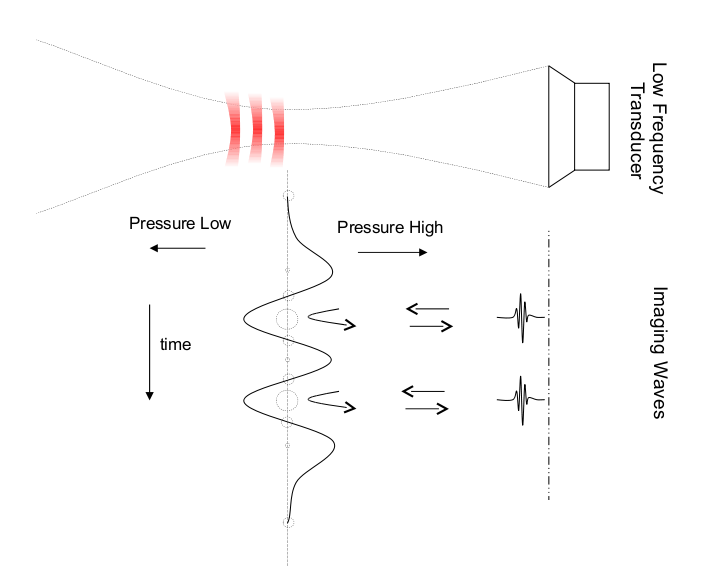
\includegraphics[width=0.8\textwidth]{change_radius.png}
%      \caption{}
% \end{figure}

% \begin{figure}[t]
%      \centering
%           \label{fig:both_waves}
%           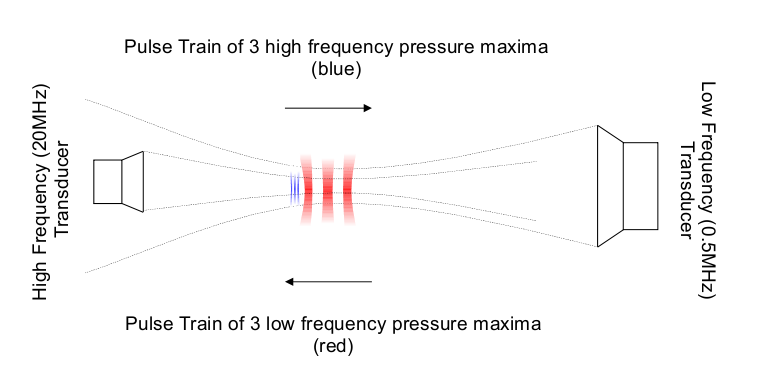
\includegraphics[width=0.8\textwidth]{both_waves.png}
%      \caption{}
% \end{figure}


% Micron-sized bubbles pulsate when insonated at diagnostic frequencies
% and thereby act as acoustic sources that add contrast to ultrasound
% images. They may be functionalised to target specific molecular
% markers but are restricted to the vasculature due to their size, which
% is hard to change. 


% For the microbubbles to  leave the blood through normal capillaries,
% we hypothesise that their size will need to be smaller than about
% 150nm.
% (See, for example, the visiculo-vacuolar transport discussed by
% \cite{Hobbs1998}).
% Tumour vasculature is more leaky with endothelial channels between
% 300-600nm being observed (\cite{Fukumori2006, Hashizume2000,
%   Hobbs1998}),
% although how rare such gaps are within the tumour vasculature is still
% somewhat of an open question (\cite{Hashizume2000}).

% Bubbles much smaller than $\frac{1}{2} \micro\metre$ are hard to manufacture.
% Without a hard stabilising coating such small bubbles dissolve within
% a fraction of a second,
% whereas with a hard shell the bubbles tend to be very stiff.
% Since the resonance frequency of a bubble increases as its radius gets smaller,
% the difficulty in producing small bubbles limits contrast agent  use to the lower resolution frequencies
% (typically below 10MHz).
% Worse still, the  restriction of contrast agents to the blood prevents ultrasound from
% developing into a fully functional imaging modality.

%and for high resolution ultrasound (10-50MHz)
%this requires sub-micron bubbles
%that are difficult to stabilise.
%Indeed, this limitation on how small bubbles can be made restricts
%microbubbles to the blood,
%for bubbles smaller  than 150nm would be required to leave
%the vasculature.

%Clinically there are problems with contrast imaging in ultrasound.
%Micron-sized bubbles seem set to remain the only
%effective method of achieving a high acoustic scattering cross-section in the
%absence of a large acoustic impedance mismatch;
%the scattering mechanism being the re-radiation of sound generated
%by a bubble induced to pulsate by the ultrasound wave,
%as opposed to a difference in the speed of sound across a boundary.
%
%after
%being induced by the ultrasound wave to pulsate
%whereby they are induced to %
%
%Bubbles have proven useful because they rely upon an entirely
%different scattering mechanism.
%They are induced to 
%pulsate by the ultrasound beam and %thereby
%re-radiate the incident sound.
%But microbubble contrast agents have their problems.
%To achieve a large scattering cross-section requires
%the bubbles to pulsate at resonance,
%and for high resolution ultrasound (10-50MHz)
%this requires sub-micron bubbles
%that are difficult to stabilise.
%Indeed, this limitation on how small bubbles can be made restricts
%microbubbles to the blood,
%for bubbles smaller  than 150nm would be required to leave
%the vasculature.

% A brief outline of the general experimental  method used  is given in \secref{Methods}.
% This will give the context not just to the experimental work,
% but also the  theoretical and computational studies.%%

% It is anticipated that there will be significant sound generated from
% when the oil first vapourises into a bubble.
% This is of interest, 
% although is not expected to be very different from previous studies of
% cavitation.
% Of greater interest is the characterisation of the  response of the  induced bubble to the
% high frequency wave.
% The problem is then to study conventional bubble imaging
% in the presence of a low-frequency wave.

% By what mechanism can the low frequency affect how the high frequency
% wave interacts with the bubble?
% There are at least two.
% %Before the study was launched, however,
% %we asked by what mechanisms we expected the low-frequency wave to
% %exert an influence.
% %We believed these to be the main mechanism.
% \desc{
%   \item[Bubble radius:]
%     The resonance frequency of a bubble is a function of
%     the bubble's equilibrium radius.
%     Due to the long wavelength of
%     the low frequency sound, in comparison to the imaging wave,
%     we can imagine it controlling the `ambient pressure' of the
%     bubble when imaged by the high-frequency wave.
%     In this way it will control the equilibrium radius of the bubble,
%     and therefore the bubble's resonance frequency.
%   \item[Bubble wall velocity:]
%     Not only will the low-frequency wave determine the radius of the
%     bubble, but
%     it will also determine the bubble's mean  radial velocity.
%     We therefore expect the bubble to be influenced by a
%     Doppler-shifted imaging frequency.
%     The magnitude of the
%     Doppler-shift will be determined by the low-frequency wave.
% }
%Firstly, the bubble will transiently be of a different radius,
%and so have a different resonance frequency.
%Secondly, the bubble wall will have a velocity and
%so the frequency experienced will be Doppler shifted from the actual
%high-frequency pulse.
%By tuning these  effects, our studies to imaging cavitating
%droplets also has a direct bearing upon high frequency bubble
%imaging.

%We hypothesise that by these effects the scattering of the high-frequency wave 
%will be dependant upon the phase of the low-frequency wave.
%This is important because scattering cross-section of a  bubble may
%then be tuned.
%At certain phases, for example,  the bubble
%will be small and shrinking, and so will have higher natural resonance
%frequency and experience a red-shifted high-frequency wave.
%    This is illustrated in \figref{general_idea}.

% Which of these effects dominate and which parameters matter?
% In what way may we tune the low-frequency wave in order to control the
% scattering of the imaging wave?
% To answer these questions we must turn to the equations that describe how the
% bubble pulsates.
%These are non-linear and so a computational study will be required.

%A further aim of the computational study is to see which of these
%mechanism dominate. 
%Is \surf\ imaging, should it work,  mainly caused by radial
%modulation, or by a Doppler shift?


%There is a problem, however.
%The equations that are commonly used to describe the bubble,
%the Rayleigh-Plesset, Herring-Trilling, Keller-Miksis equations, for
%example,
%do not contain a Doppler effect.
%It is `missing' from the model, 
%even though intuitively it ought to be there.



%  There is a problem, however.
%  The equations that are commonly used to describe the bubble,
%  the Herring-Trilling and Keller-Miksis equations%  Rayleigh-Plesset,
%  , for
%  example,
% % are awkward since their formulation as differential
% % equations, that can be solved only numerically, makes the Doppler-influence hard to study.
% % Indeed, 
% % that there is a Doppler-effect contained within these equations at all
% % is easily missed, 
% % and perhaps this is why the Doppler-contribution to bubble wall motion
% % has not as-of-yet, to the author's knowledge, been studied.


% study differential equations for which 
% have the 
% elation the influence of the Doppler effect.
% The influence is felt in the numerical computation of the equations,
% but it is hard, analytically to delineate it's contribution.

%do not contain a Doppler effect.
%It is `missing' from the model, 
%even though intuitively is ought to be there.
%Furthermore the equations do not `break' when the bubble wall velocity
%exceeds the speed of sound. 

%The Keller-Miksis equation models the radial oscillations of the
%bubble that
%will contribute to the the  far field acoustic wave.
%The validity of the equation at high bubble wall velocities (i.e. near
%the speed of sound, speeds that the bubble wall routinely reach) has been questioned, however
%(\cite{Prosperetti1986}).
%On the one hand, the equation does not break down as it should when the wall
%velocity equals the speed of sound and so it is argued that the
%description when shock waves are present is incorrect.
%On the other hand, however, 
%On the other hand,

%The equations that are commonly used to describe the bubble,
%the Rayleigh-Plesset, Herring-Trilling, Keller-Miksis equations for
%example,
%do not contain a Doppler effect.
%It is `missing' from the model, 
%even though intuitively is ought to be there.
%Furthermore the equations do not `break' when the bubble wall velocity
%exceeds the speed of sound. 

%Since the bubble wall velocity routinely reaches the same order as the speed
%of sound in microbubble physics,
%the resolotuion to this query is required.
%This can be done by deriving the acoustic output of a bubble using the
%older and 
%more general theory of  `aerodynamic' sound.
%This theory was originally  developed in the 1950s to describe the
%acoustic output of jet engines,
%and the general problem of finding the acoustic output of fast moving
%surfaces was solved by \cite{FfowcsWilliams1969}.


%To resolve whether or not the Keller-Miksis equation applies high
%bubble wall velocities, we can compare it with a model especially
%designed for sit the model in a more general setting 
%predictions of , 
%To resolve this, as well as other problems (introduced below), 
%a new equation to describe the bubble wall motion needs to be developed.
%The outline for how this is done is given in \secref{KellerModel}, borrowing heavily from the
%`aerodynamic' theory of sound originally developed in the 1950s to describe the
%acoustic output of jet engines.

%of bubble wall motion that would be used to answer such
%a question (The Rayleigh-Plesset, Herring-Trilling, Keller-Miksis models,
%for example) do not contain a Doppler effect.
%It is missing from the model, even though intuitively, the
%Doppler-effect on the bubble should certainly be there.
%It is missing, however, from the equations generally used to model  bubble wall
%motion (The Rayleigh-Plesset, Herring-Trilling, Keller-Miksis models,
%for example).
%We cannot n


%There is much that can potentially be learned from this dual wave
%approach.

%all the experimental work has been small variations on a common setup.
%To solve the questions raised by these experiments,
%the setup has also influenced the theoretical and particularly
%computational aspects of the project.
%We therefore give an outline first.

%Putting to one side temporally the problem of cavitating the oil,

% A more stable and better understood source of bubbles are those that
% are manufactured commercially for ultrasound imaging.
% We therefore began the experimental work by studying Levovist and Sonovue to
% determine the influence of the low frequency wave on high frequency
% imaging.
% This technique of using a low frequency wave to alter the
% scattering-cross section of a higher frequency wave often goes by the
% name of \surf\ imaging and some experimental results are given
% in \secref{bubble_exp}.

%and is the source of ongoing experimental work.

%As will be seen in \secref{bubble_exp},
%the preliminary  study into \surf\ imaging could not determine a
%strong influence of the low frequency wave.
%To understand why this is, and to try to narrow the viable experimental
%parameters, a computational study was launched.
%The aims of this study were to determine pressures and frequency that
%should be used to obtain the strongest 
%influence of the low frequency wave on the imaging wave.


%\section{Literature Review}


%%% Local Variables: 
%%% mode: latex
%%% TeX-master: "../../tshorrock_thesis"
%%% End: 
